\scanpage{52}
$M$ \uline{plat} cela est-il une propriété typique [elle est stable par $\varinjlim$ \unsure{filtr|filtr.} et par chgt de topos $\}$

\[
 N\longmapsto M\otimes N\quad\text{exact}
\]
$\forall\ f_1$ -- $f_n$ sections de $A$ sur $U$,
\[
 (\textstyle\sum f_i A)\otimes M\longrightarrow M\quad\text{injectif}
\]
Il suffit de l'exiger \deleted{pour} les \inserted{\unsure{syst. de}} sections \unsure{universel|universelles}, i.e. $U\unsure{:=|=} A^n$
\[
 (\textstyle\sum t_i A_{U_n})\otimes M_{U_n}\longrightarrow M_{U_n}\quad\text{injectif.}
\]
\[
 U_n=A^n
\]
\diagram{\begin{tikzcd}[ampersand replacement=\&,column sep=small,row sep=small]
 M\arrow[d,dashed,no head]\arrow[r,dashed] \& M_i\\
 Y\arrow[dr] \& Y_i\arrow[l]\\
 \& N,\text{ plat}\\
 Z\arrow[uu,bend left=18] \&
\end{tikzcd}
\qquad
\begin{tikzcd}[ampersand replacement=\&,row sep=small,column sep=small]
 M\arrow[r] \& \unsure{M'|M_i} \&\\
 A\arrow[r]\arrow[drr,no head] \& \unsure{A'|A_i} \& N\,\text{plat}\arrow[d,no head]\\
 \& \& B
\end{tikzcd}}

\diagram{\begin{tikzcd}[ampersand replacement=\&]\mathbf Y\&\mathbf X\arrow[l]\end{tikzcd}}

\figure{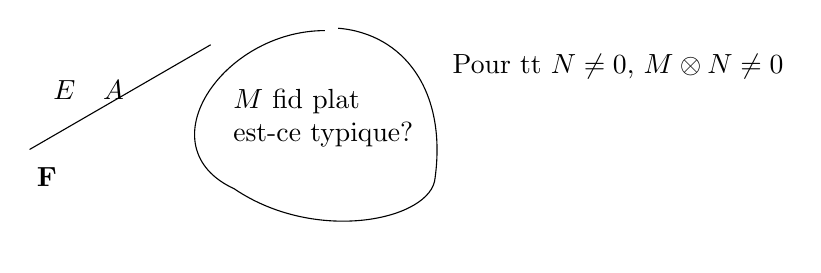
\begin{tikzpicture}
\node at (0,.2) {$E\quad A$};\draw (-.75,-.55) -- (1.55,.78);
\node at (-.53,-.9) {$\mathbf F$};
\draw (3,.96) .. controls (1.7,.96) and (.7,-.52) .. (1.85,-1.05) .. controls (2.9,-1.76) and (4.36,-1.44) .. (4.4,-.91) .. controls (4.55,.2) and (4,.92) .. (3.17,.99);
\node[align=left] at (2.98,-.15) {$M$ \uuline{fid} \uline{plat}\\est-ce typique?};
\node[anchor=west] at (4.5,.5) {Pour tt $N\ne 0$, $M\otimes N\ne 0$};
\end{tikzpicture}}

$\mathbf E_{\mathbf A}$\qquad \uuline{Modpf} $(A)$ champ des modules de p.f. sur $A$
\[
 \underline{\operatorname{Hom}}\bigl(\text{\uuline{Modpf}}(A),\text{\uuline{Fl}}(E)\bigr)
 \qquad\text{Catégorie des hom de Champs \unsure{de|des}}
\]
\deleted{les objets}
\[
 \begin{aligned} E&\longrightarrow F& &\text{hom. de champs \uline{constants}}\\
 &&M&\longmapsto X \end{aligned}
\]
d'où \quad $A_{\mathbf F}$ \qquad $\mathbf R$

\uline{Algèbres}
\diagram{$\displaystyle\left.\begin{array}{l}
 \text{\deleted{de} t.f}\\ \text{p.f.}\\ \text{lisses}\\ \text{étales}\\ \text{nettes}
 \end{array}\right]\quad
 \begin{array}{l}\text{\unsure{$\leftarrow$}}\\\text{peu typiques}\\\text{car ne \unsure{commut|commutent} pas}\\\text{aux }\underrightarrow{\lim}\end{array}$}

\diagram{$\left|\begin{array}{ll}
 \text{\uline{radicielles} / monomorphiques} & \deleted{\unsure{\rm OK}}\ \text{OK, par prod. fibrés.}\\
 \boxed{\text{\uline{surjectives} \unsure{?|X|?!}}} &\\
 \text{plates}^{\text{OK}}\text{ / fid plates}&\\
 \text{formellmt lisse}&\\
 \text{--- net}&\text{OK}\\
 \text{--- étale}&\\
 \text{entières}&\text{OK}\\
 \text{homéo. universels}&
 \end{array}\right.$}

\margin{Considérons une Algèbre qui est déjà de \uuline{\deleted{\unsure{t}}p.f.} On veut ``la \unsure{vendre|rendre}'' plate, ou lisse etc. Cela se fait-il par un sous-topos ??}
% archive sheet number: 51
